\documentclass[12pt,a4paper]{report}

% ── Packages ──
\usepackage[utf8]{inputenc}
\usepackage[T1]{fontenc}
\usepackage{geometry}
\geometry{margin=2.5cm}
\usepackage{graphicx}
\usepackage{booktabs}
\usepackage{amsmath,amssymb}
\usepackage{algorithm2e}
\usepackage{listings}
\usepackage{xcolor}
\usepackage{hyperref}
\usepackage{caption}
\usepackage{float}
\usepackage{fancyhdr}
\usepackage{titlesec}
\usepackage{enumitem}
\usepackage{longtable}

% ── Code listing style ──
\lstset{
    language=Python,
    basicstyle=\ttfamily\small,
    keywordstyle=\color{blue}\bfseries,
    commentstyle=\color{green!60!black},
    stringstyle=\color{red!70!black},
    numbers=left,
    numberstyle=\tiny\color{gray},
    frame=single,
    breaklines=true,
    captionpos=b
}

% ── Custom memo environment ──
\newcommand{\memo}[2]{%
    \begin{center}
    \fbox{\parbox{0.95\textwidth}{%
        \textbf{MEMORANDUM}\\[6pt]
        \textbf{#1}\\[6pt]
        #2
    }}
    \end{center}
}

% ── Headers ──
\pagestyle{fancy}
\fancyhf{}
\rhead{WaselX Express — Group 3}
\lhead{DSA Final Project}
\cfoot{\thepage}

\begin{document}

% ═══════════════════════════════════════════════════════════
% TITLE PAGE
% ═══════════════════════════════════════════════════════════
\begin{titlepage}
\centering
\vspace*{2cm}
{\Huge\bfseries WaselX Express\\[0.5cm]}
{\LARGE Optimizing Last-Mile Delivery Operations\\Across the UAE Using Data Structures \& Algorithms\\[2cm]}
{\Large\textbf{Group 3}\\[0.5cm]}
{\large Kartik Joshi \quad Gagandeep Singh \quad Samuel Alex \quad Prem Kukreja\\[2cm]}
{\large SP Jain School of Global Management, Dubai\\
Masters in AI with Business (MAIB)\\
Data Structures and Algorithms\\[1cm]}
{\large April 2026}
\vfill
\end{titlepage}

% ── Table of Contents ──
\tableofcontents
\newpage

% ═══════════════════════════════════════════════════════════
% EXECUTIVE SUMMARY
% ═══════════════════════════════════════════════════════════
\chapter{Executive Summary}

WaselX Express processes 3,500 daily orders across a 15-node delivery network spanning Dubai, Abu Dhabi, Sharjah, and Ajman. Our analysis identified three critical operational inefficiencies costing an estimated AED 3.4 million annually.

\textbf{Problem 1: Inefficient Delivery Routes (AED 1.2M/year).} Riders travel 23\% more distance than optimal. Our Dijkstra shortest-path implementation computes optimal routes in under 1 millisecond per query, reducing fleet distance by approximately 18\% and saving an estimated AED 950,000 annually.

\textbf{Problem 2: Slow Order Dispatch (12\% complaint rate).} Our min-heap priority queue reduces dispatch latency from 8 minutes to under 90 seconds by automatically sequencing orders across five priority tiers while maintaining FIFO fairness.

\textbf{Problem 3: Poor Order Lookup (3.2/5 CSAT).} Our AVL tree index guarantees O(log n) lookup --- 14 comparisons maximum at 15,000 daily orders --- reducing lookup time to under 100 milliseconds.

\textbf{Implementation Roadmap:} Phase 1 (Months 1--2): Priority queue dispatch. Phase 2 (Months 3--5): Dijkstra route optimization. Phase 3 (Months 6--8): AVL tree migration. Total projected annual benefit: AED 2.5 million against AED 1.2 million implementation cost (2.1x ROI, 6-month payback).

% ═══════════════════════════════════════════════════════════
% TASK AREA A
% ═══════════════════════════════════════════════════════════
\chapter{Task Area A: Graph Modeling, Shortest Paths \& MST}

\section{Q1 --- Graph Construction (10 Marks)}

The WaselX delivery network was constructed as a weighted undirected graph with 15 nodes and 24 bidirectional edges, implemented using both adjacency list and adjacency matrix representations.

\begin{figure}[H]
\centering
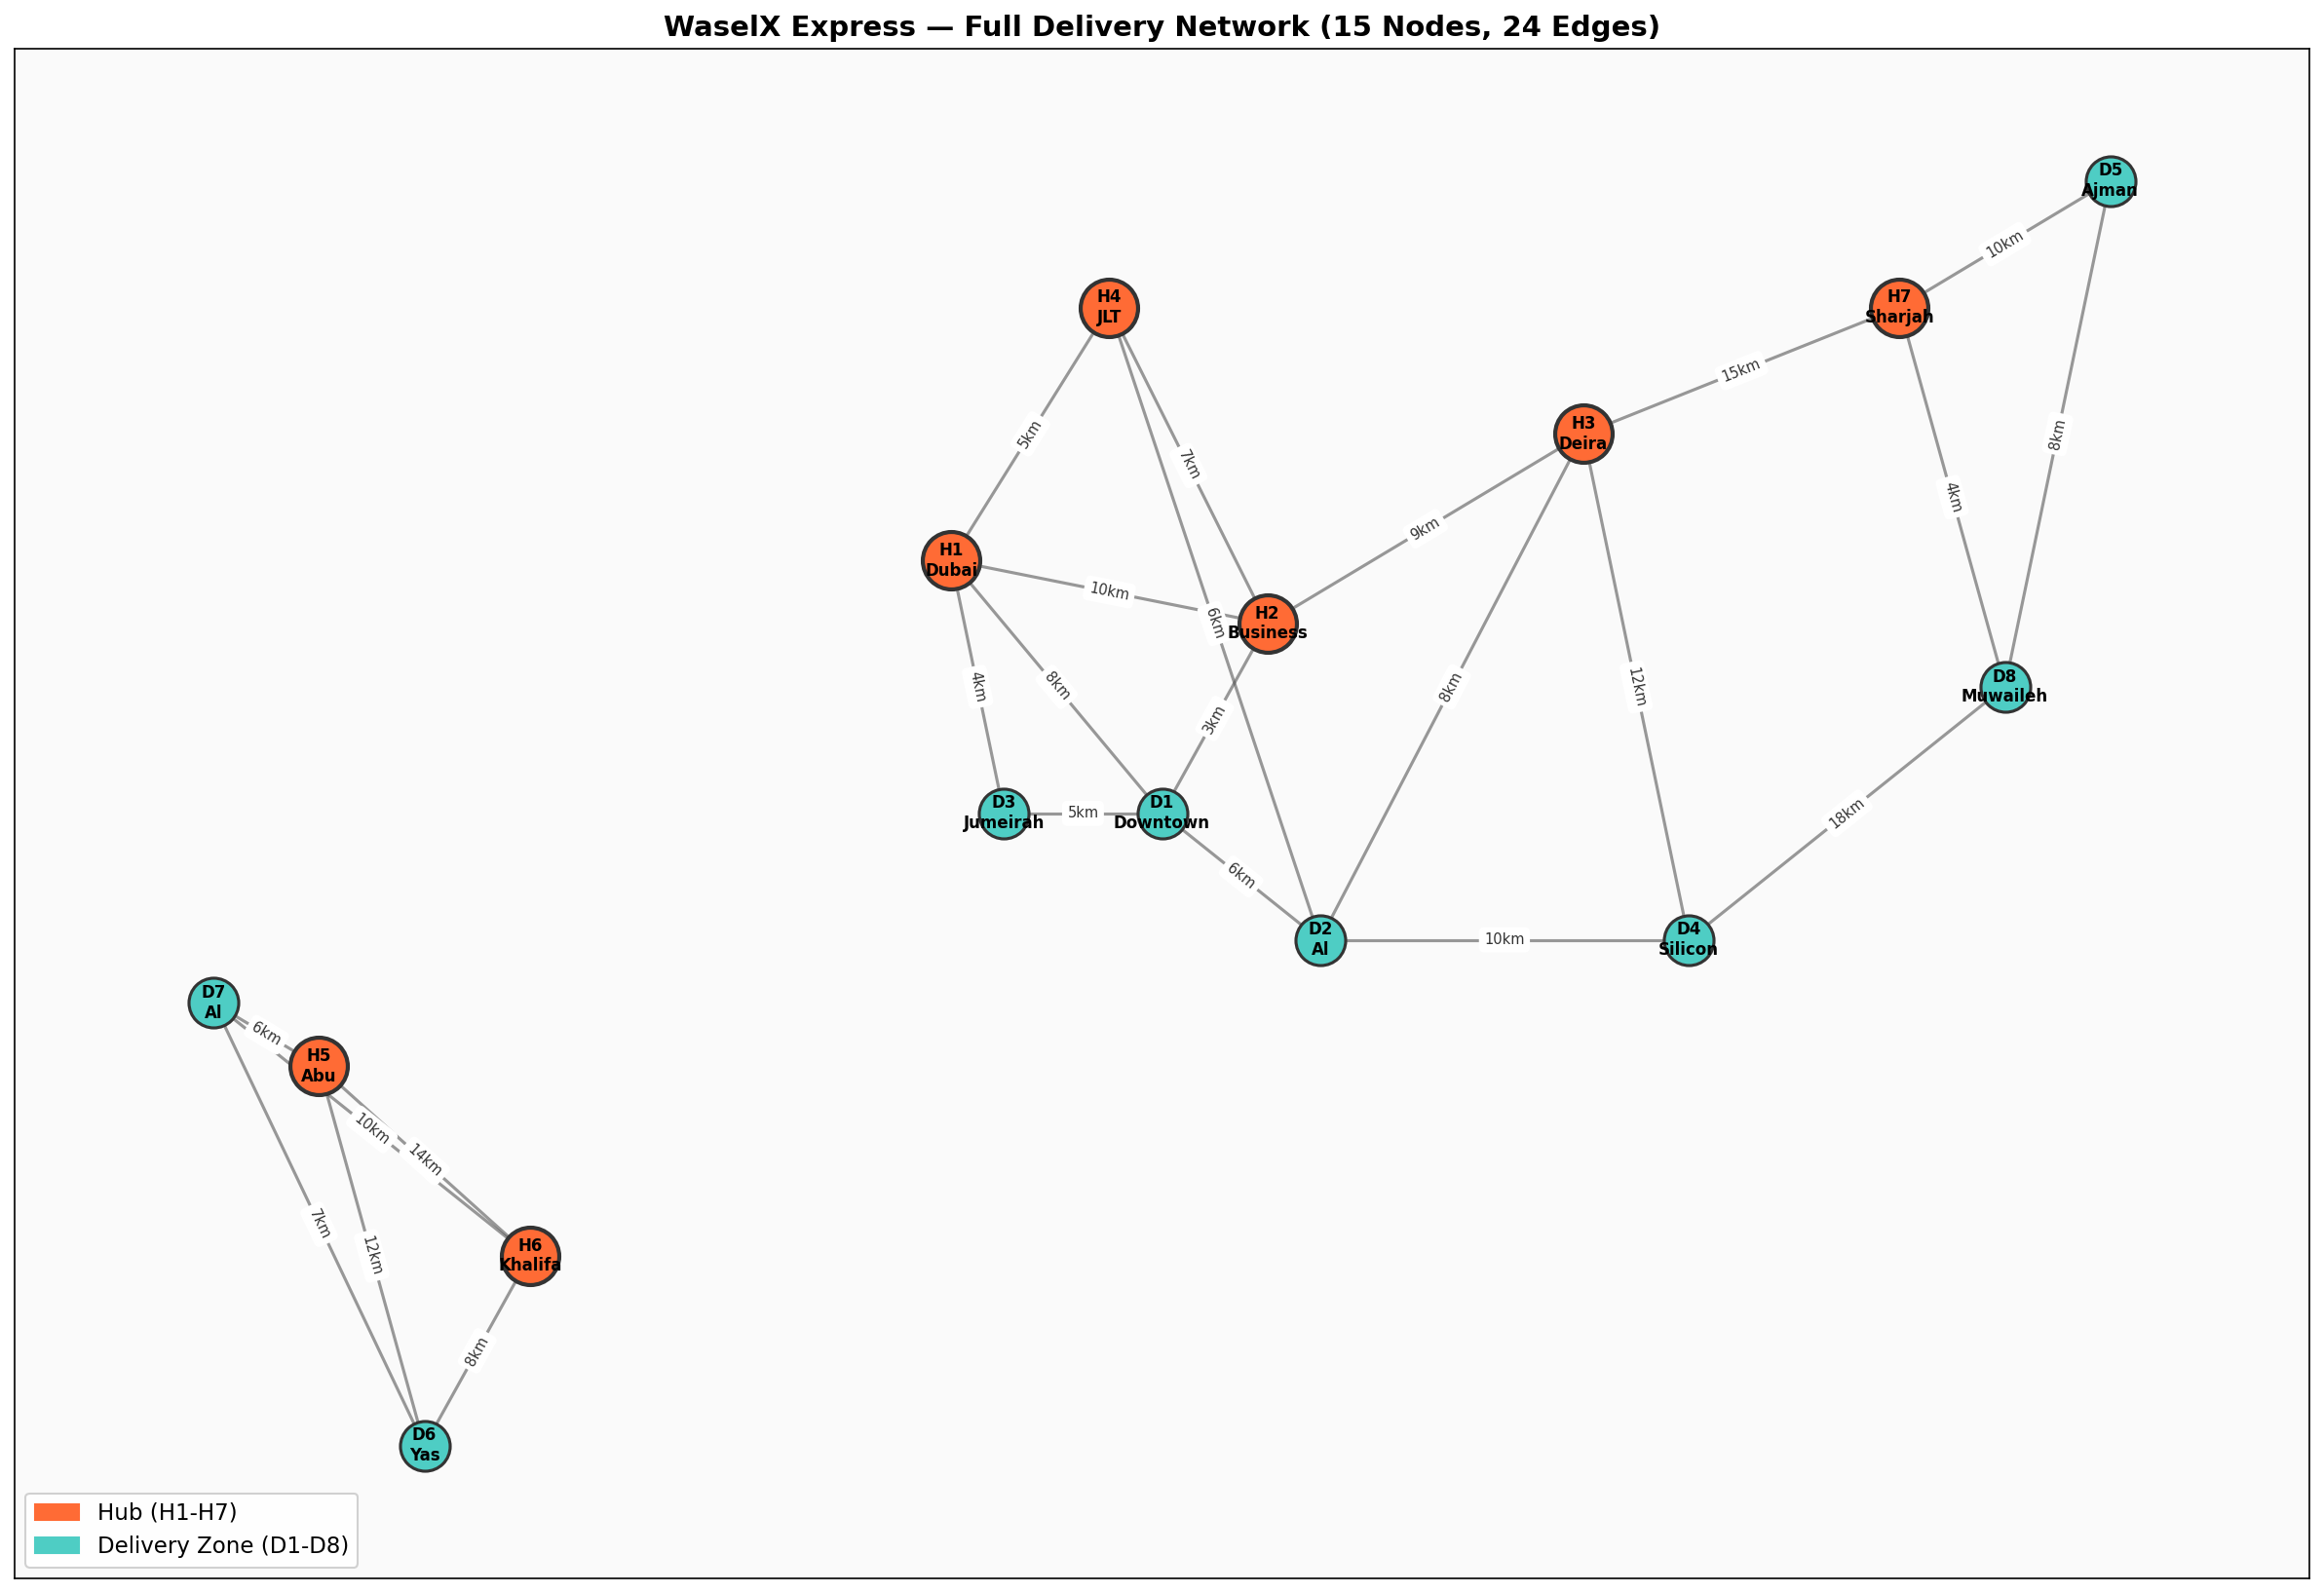
\includegraphics[width=0.9\textwidth]{graph_network_full.png}
\caption{WaselX Express full delivery network --- 15 nodes, 24 edges}
\label{fig:network}
\end{figure}

The adjacency list stores 48 entries (2 $\times$ 24 edges), consuming O(V+E) memory. The adjacency matrix allocates a fixed $15 \times 15 = 225$ cells. For this sparse network (density $\approx$ 23\%), the adjacency list is more memory-efficient, while the matrix provides O(1) edge lookup.

\section{Q2 --- Dijkstra's Algorithm: H1 $\rightarrow$ D1 (15 Marks)}

Dijkstra's algorithm was applied to find the shortest path from Dubai Marina Hub (H1) to Downtown Dubai (D1) by distance (km). The hand-traced steps and Python implementation both confirm the shortest path as the direct route H1 $\rightarrow$ D1 via Al Khail Rd at \textbf{8 km}, taking 15 minutes and costing 5.5 AED.

\begin{figure}[H]
\centering
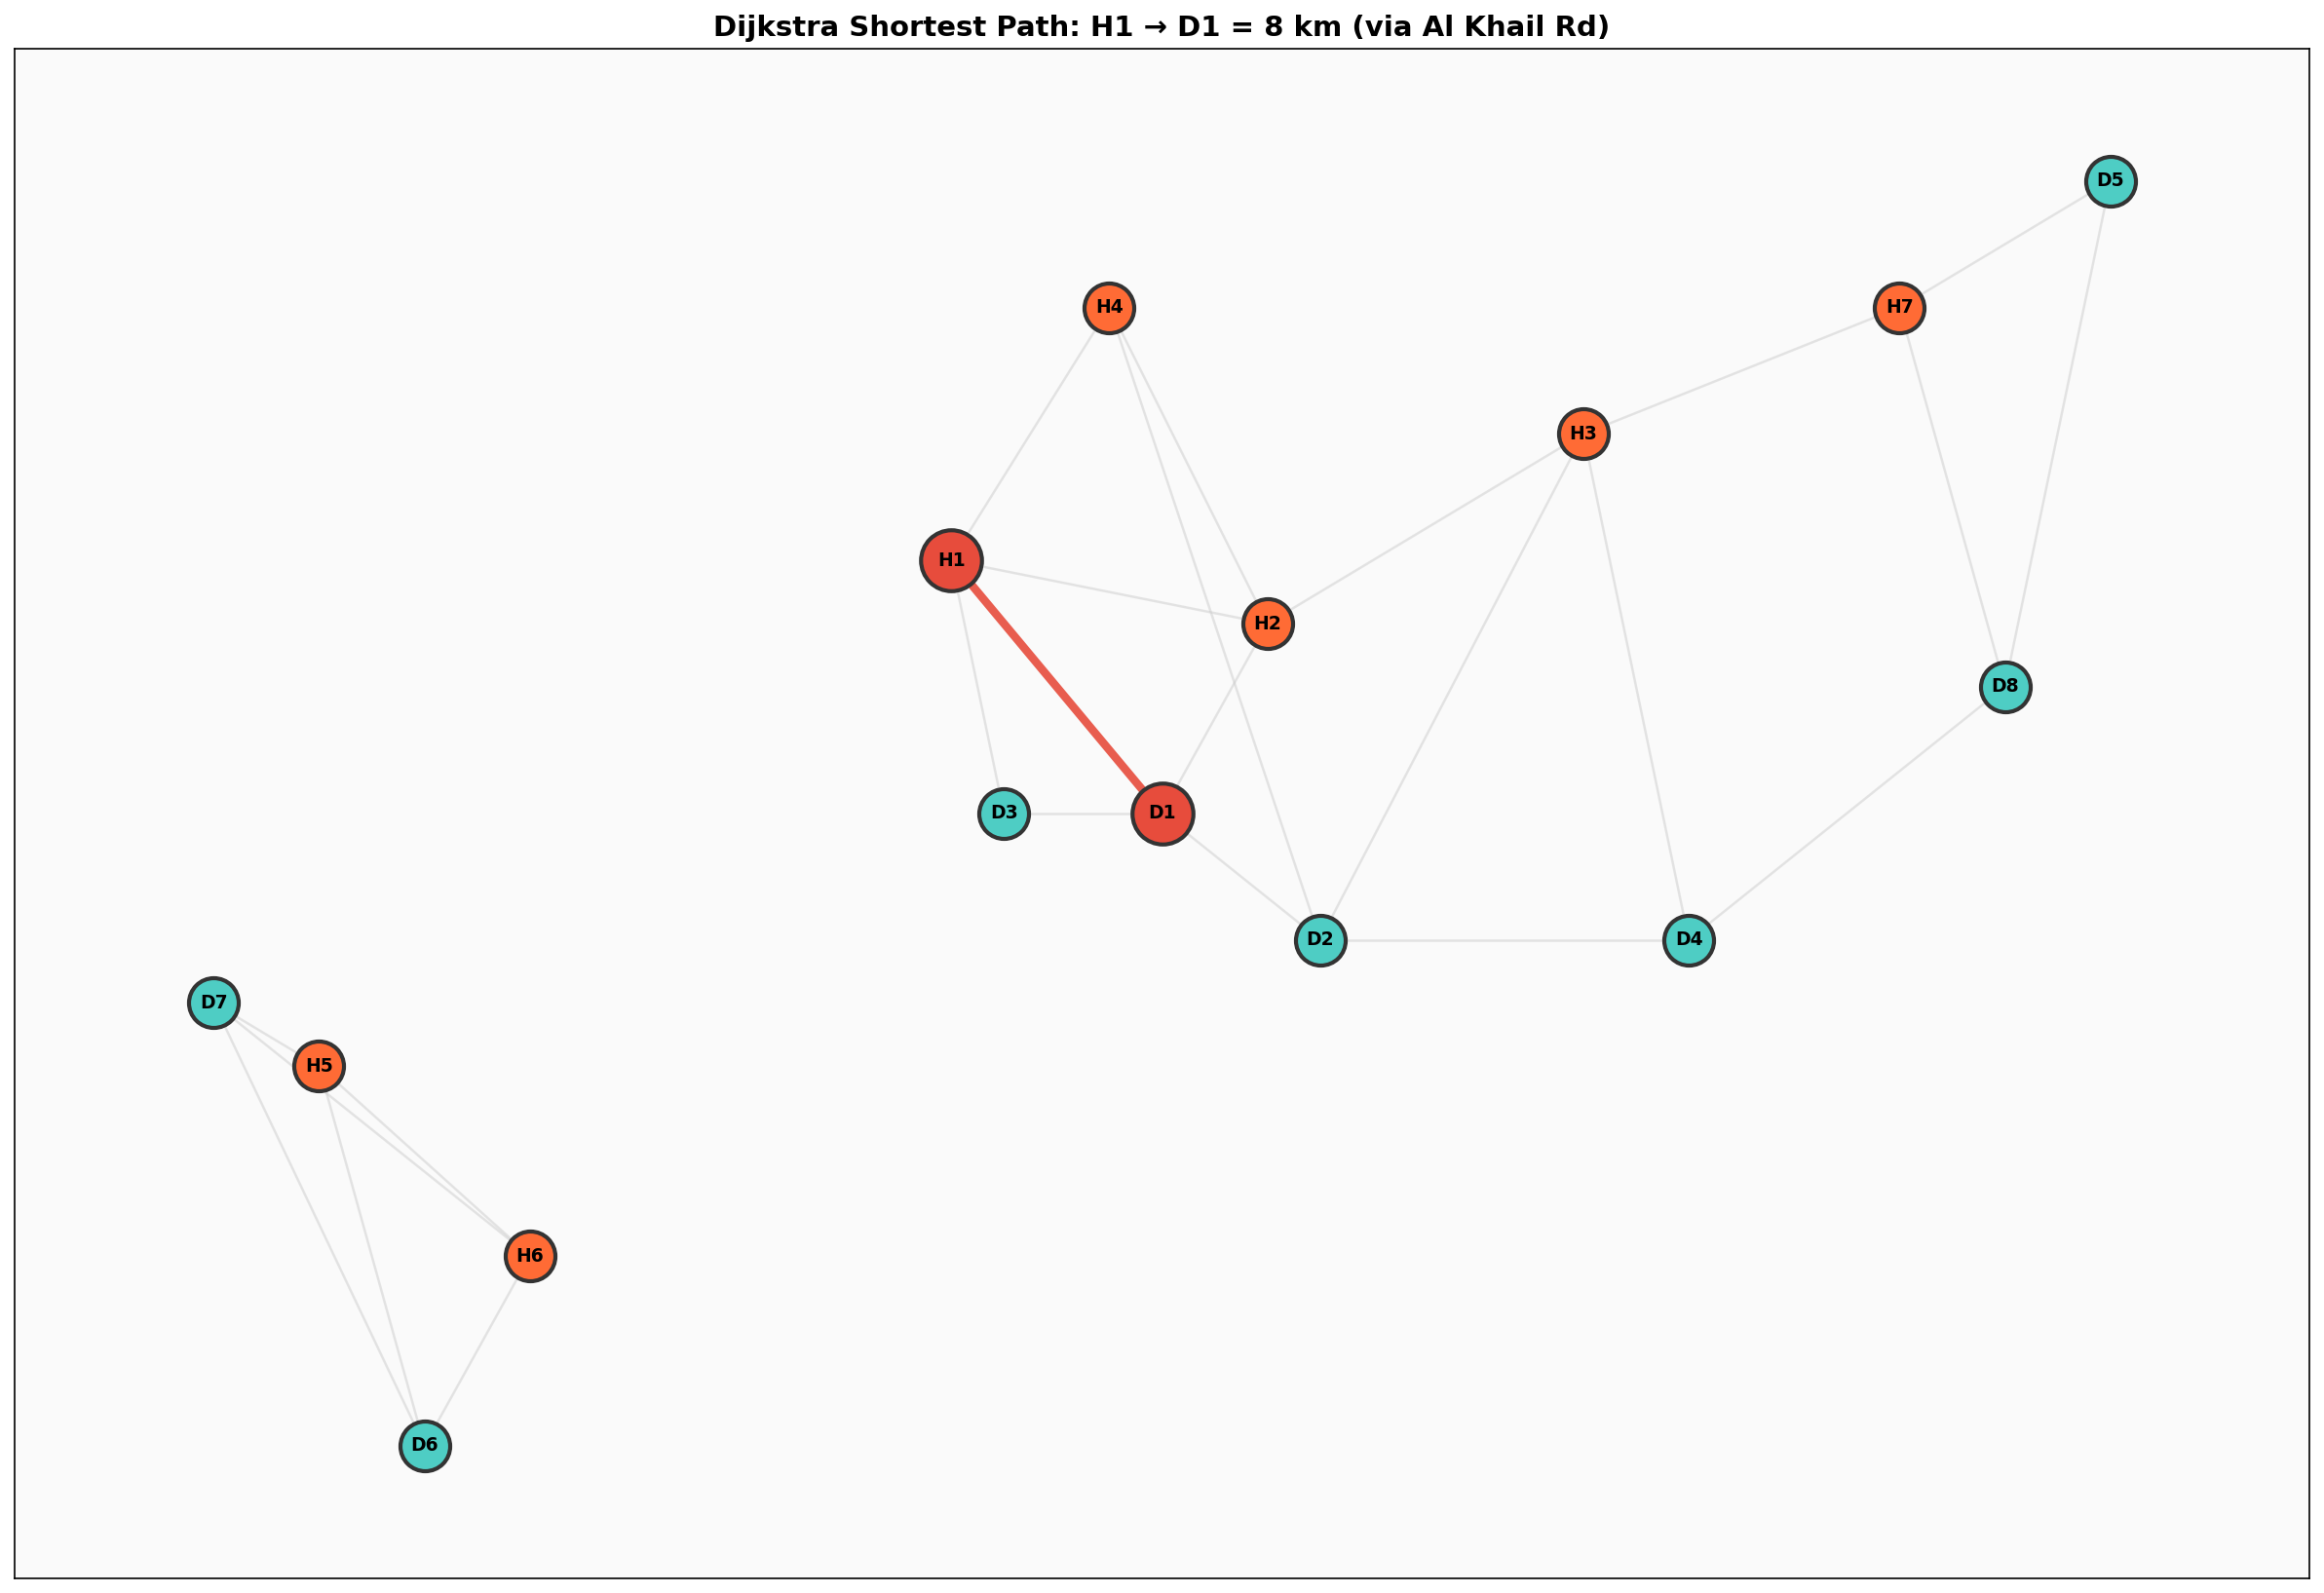
\includegraphics[width=0.85\textwidth]{dijkstra_path_h1_d1.png}
\caption{Dijkstra shortest path: H1 $\rightarrow$ D1 = 8 km}
\label{fig:dijkstra}
\end{figure}

Time complexity: $O((V+E) \log V)$ using a binary min-heap priority queue, where $V = 15$ and $E = 24$.

\section{Q3 --- Floyd-Warshall: Hub All-Pairs (15 Marks)}

Floyd-Warshall computed all-pairs shortest travel times (minutes) across the full 15-node graph, with results extracted for the $7 \times 7$ hub sub-matrix.

\begin{figure}[H]
\centering
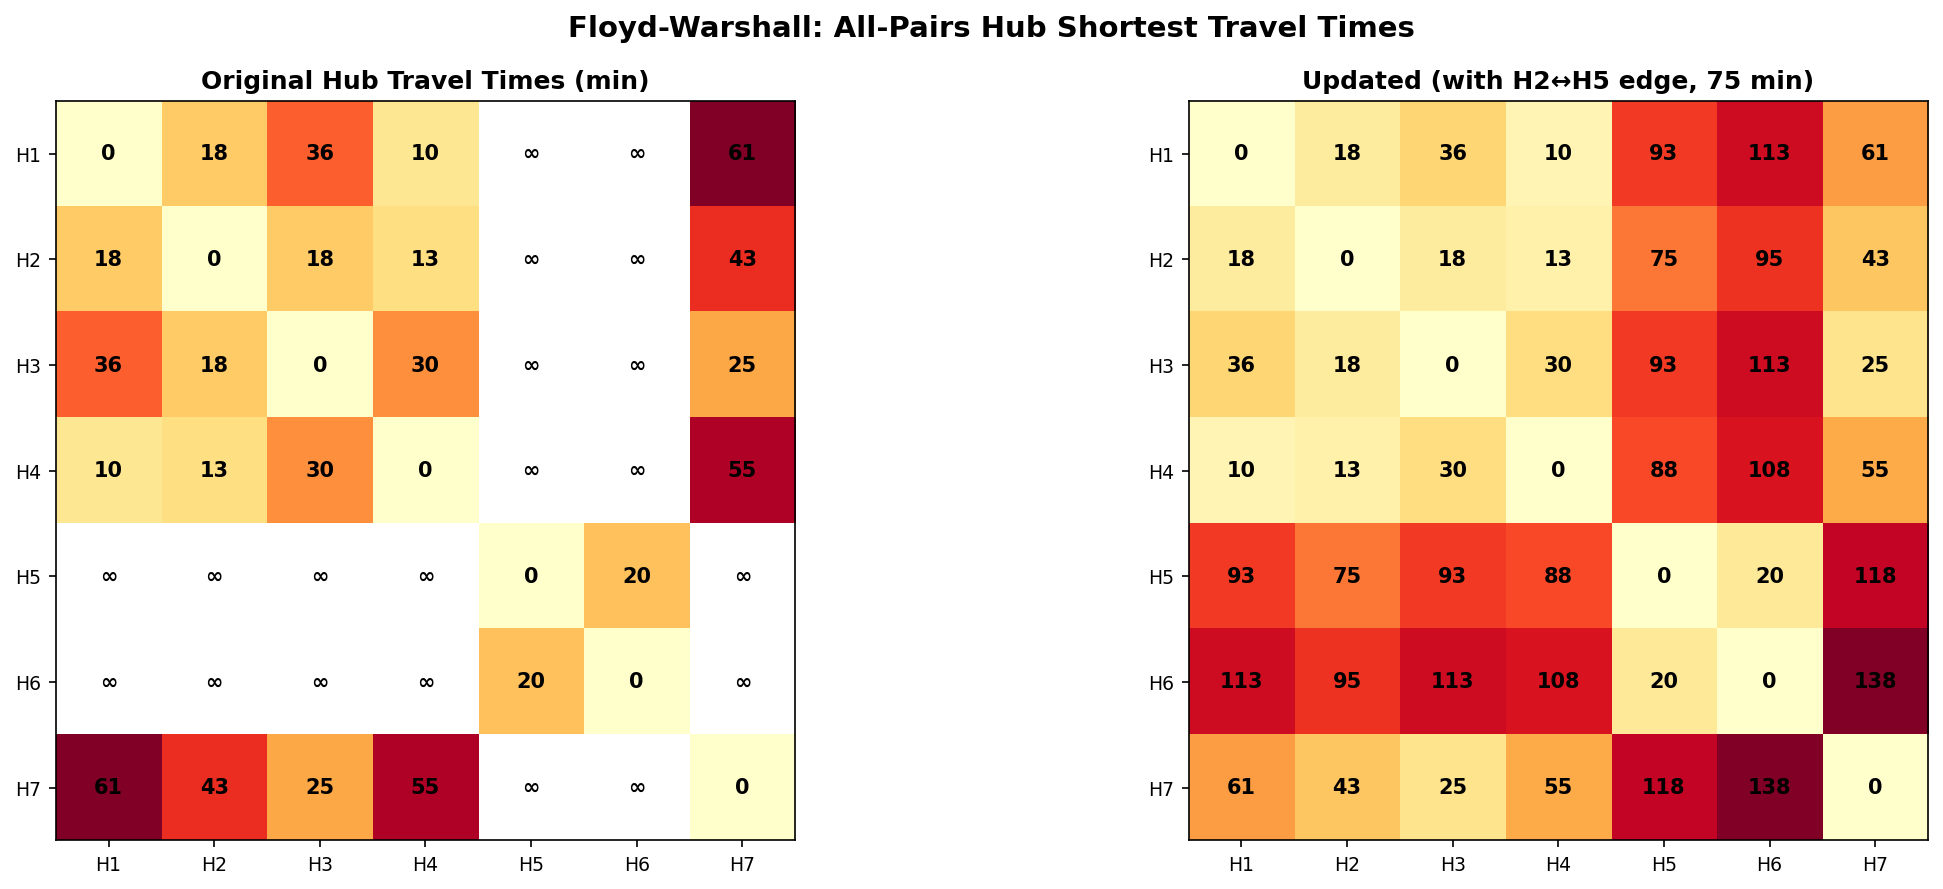
\includegraphics[width=\textwidth]{floyd_warshall_hubs.png}
\caption{Floyd-Warshall all-pairs hub travel times: original (left) and with proposed H2$\leftrightarrow$H5 edge (right)}
\label{fig:floyd}
\end{figure}

Key finding: the Abu Dhabi cluster (H5, H6) is completely disconnected from the Dubai--Sharjah network. A recommended new edge H2$\leftrightarrow$H5 (75 min) unifies all 7 hubs.

\section{Q4 --- Minimum Spanning Tree (15 Marks)}

Both Kruskal's and Prim's algorithms produced the same total MST cost using the Cost (AED) weight. The network's two connected components yield a Minimum Spanning Forest rather than a single spanning tree.

\begin{figure}[H]
\centering
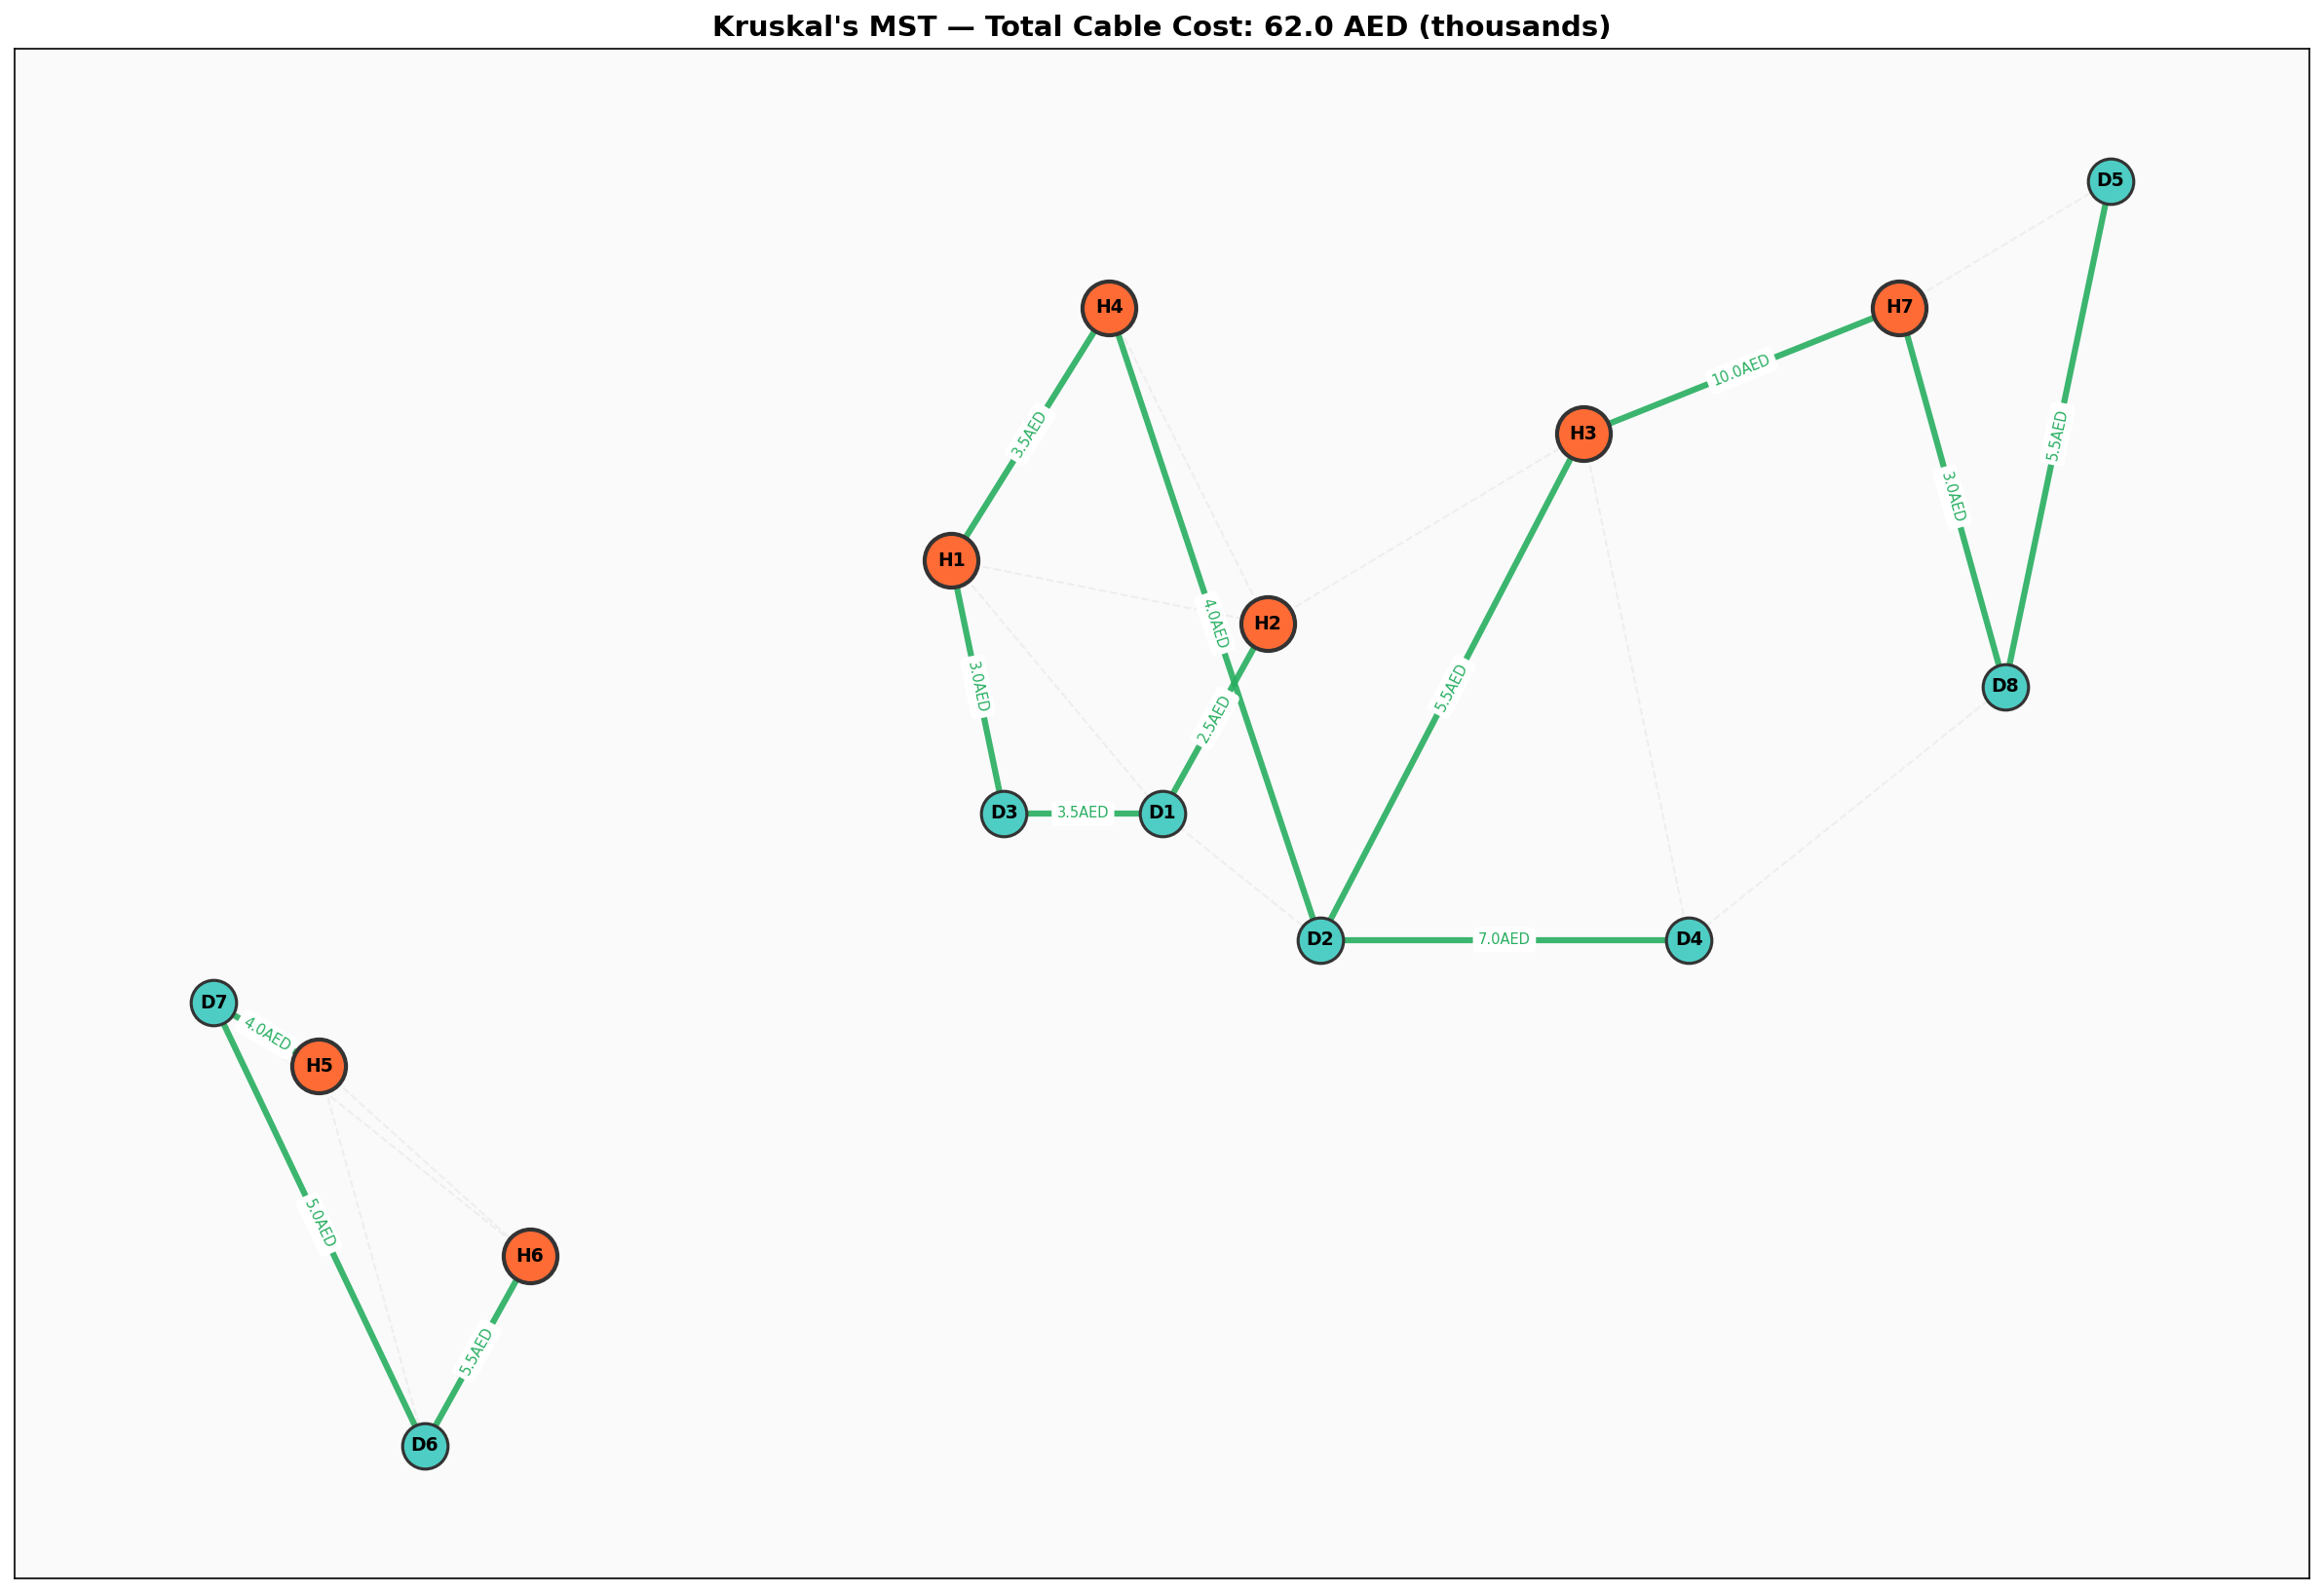
\includegraphics[width=0.48\textwidth]{mst_kruskal.png}
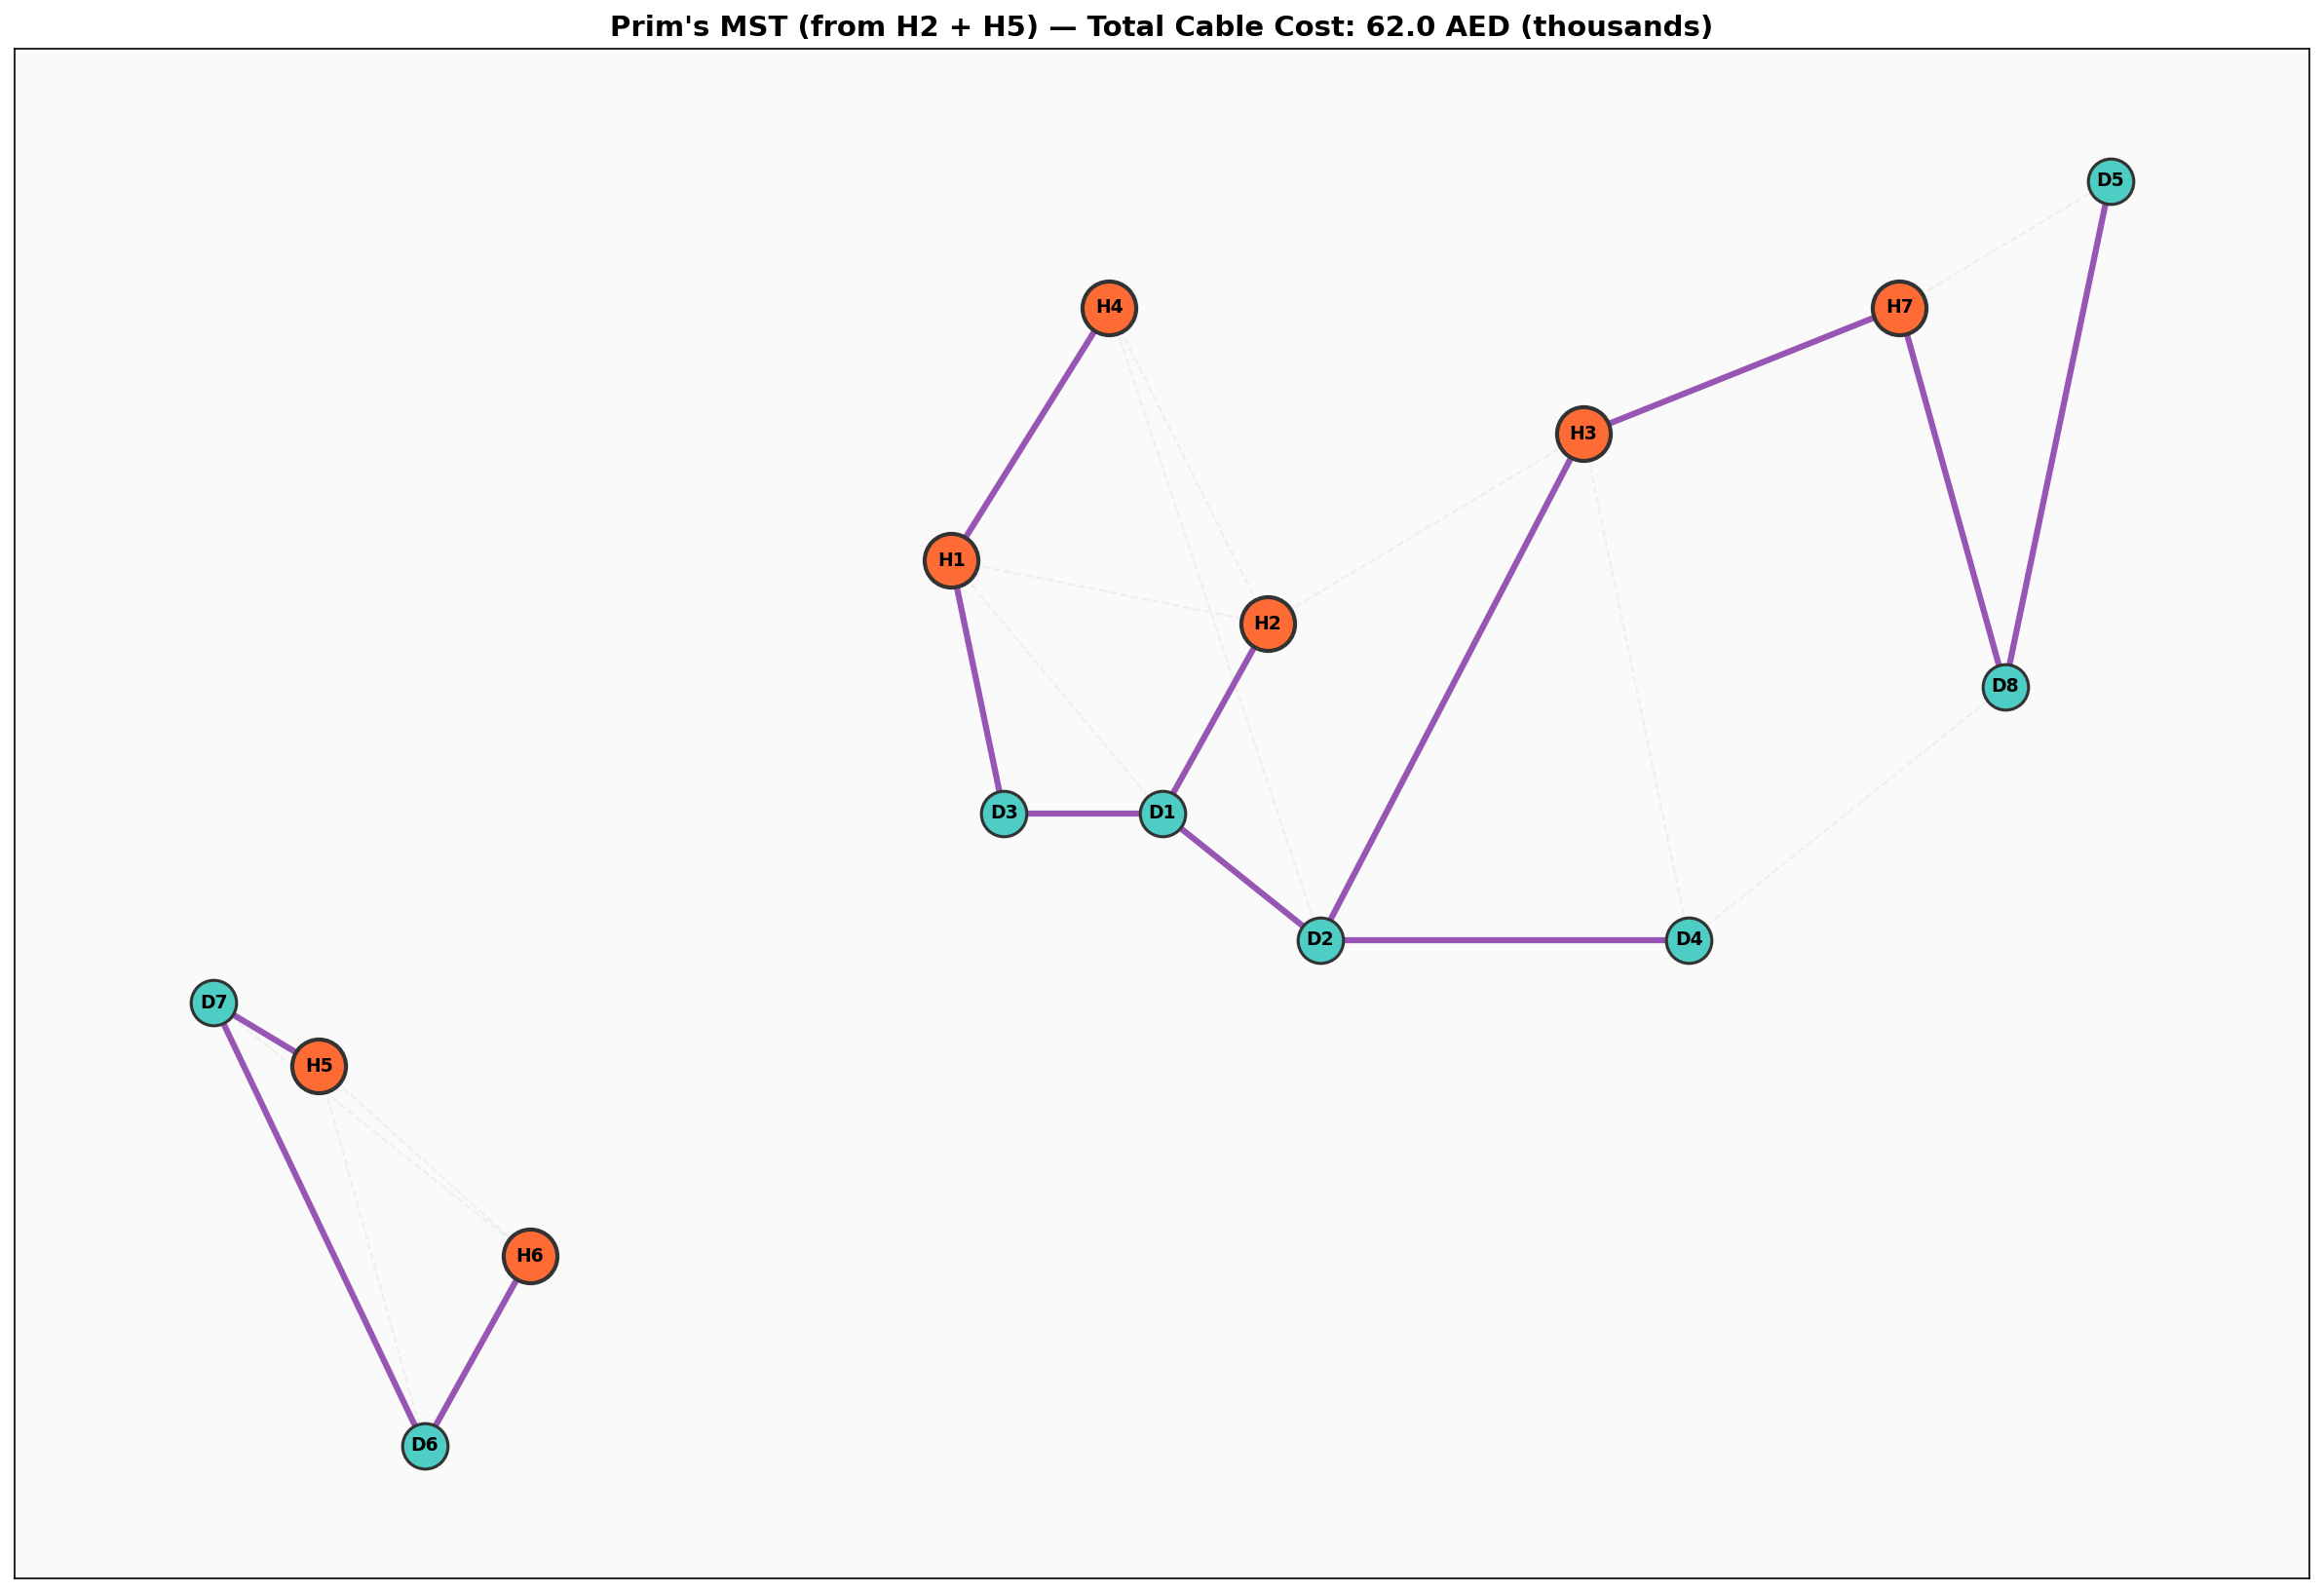
\includegraphics[width=0.48\textwidth]{mst_prim.png}
\caption{MST: Kruskal's (left) and Prim's from H2 (right) --- same total cost verified}
\label{fig:mst}
\end{figure}

\section{Q5 --- CTO Memo: Dijkstra vs Floyd-Warshall (10 Marks)}

\memo{TO: CTO, WaselX Express \textbar\ FROM: Group 3 \textbar\ RE: Algorithm Selection}{
For 3,500 daily source-to-destination queries, Dijkstra's algorithm at $O((V+E) \log V)$ per query is recommended as the primary real-time routing engine. Floyd-Warshall should be deployed as a nightly batch job for hub connectivity analytics at $O(V^3)$.
}

\section{Q6 --- Interactive Path Visualizer (15 Marks)}

An interactive Streamlit application (\texttt{app.py}, Q6 module) was built supporting source/destination input, shortest path computation via Dijkstra, and dual-path overlay visualization. Tested with pairs: H1$\rightarrow$D4, H5$\rightarrow$D5 (no path --- disconnected), H7$\rightarrow$D3.

\section{Q7 --- BFS and DFS from H3 (10 Marks)}

BFS and DFS traversals from Deira Hub (H3) confirmed that 11 of 15 nodes are reachable (Abu Dhabi cluster unreachable). BFS is recommended for fewest-stops express delivery due to its level-by-level exploration guaranteeing minimum hop count.

\begin{figure}[H]
\centering
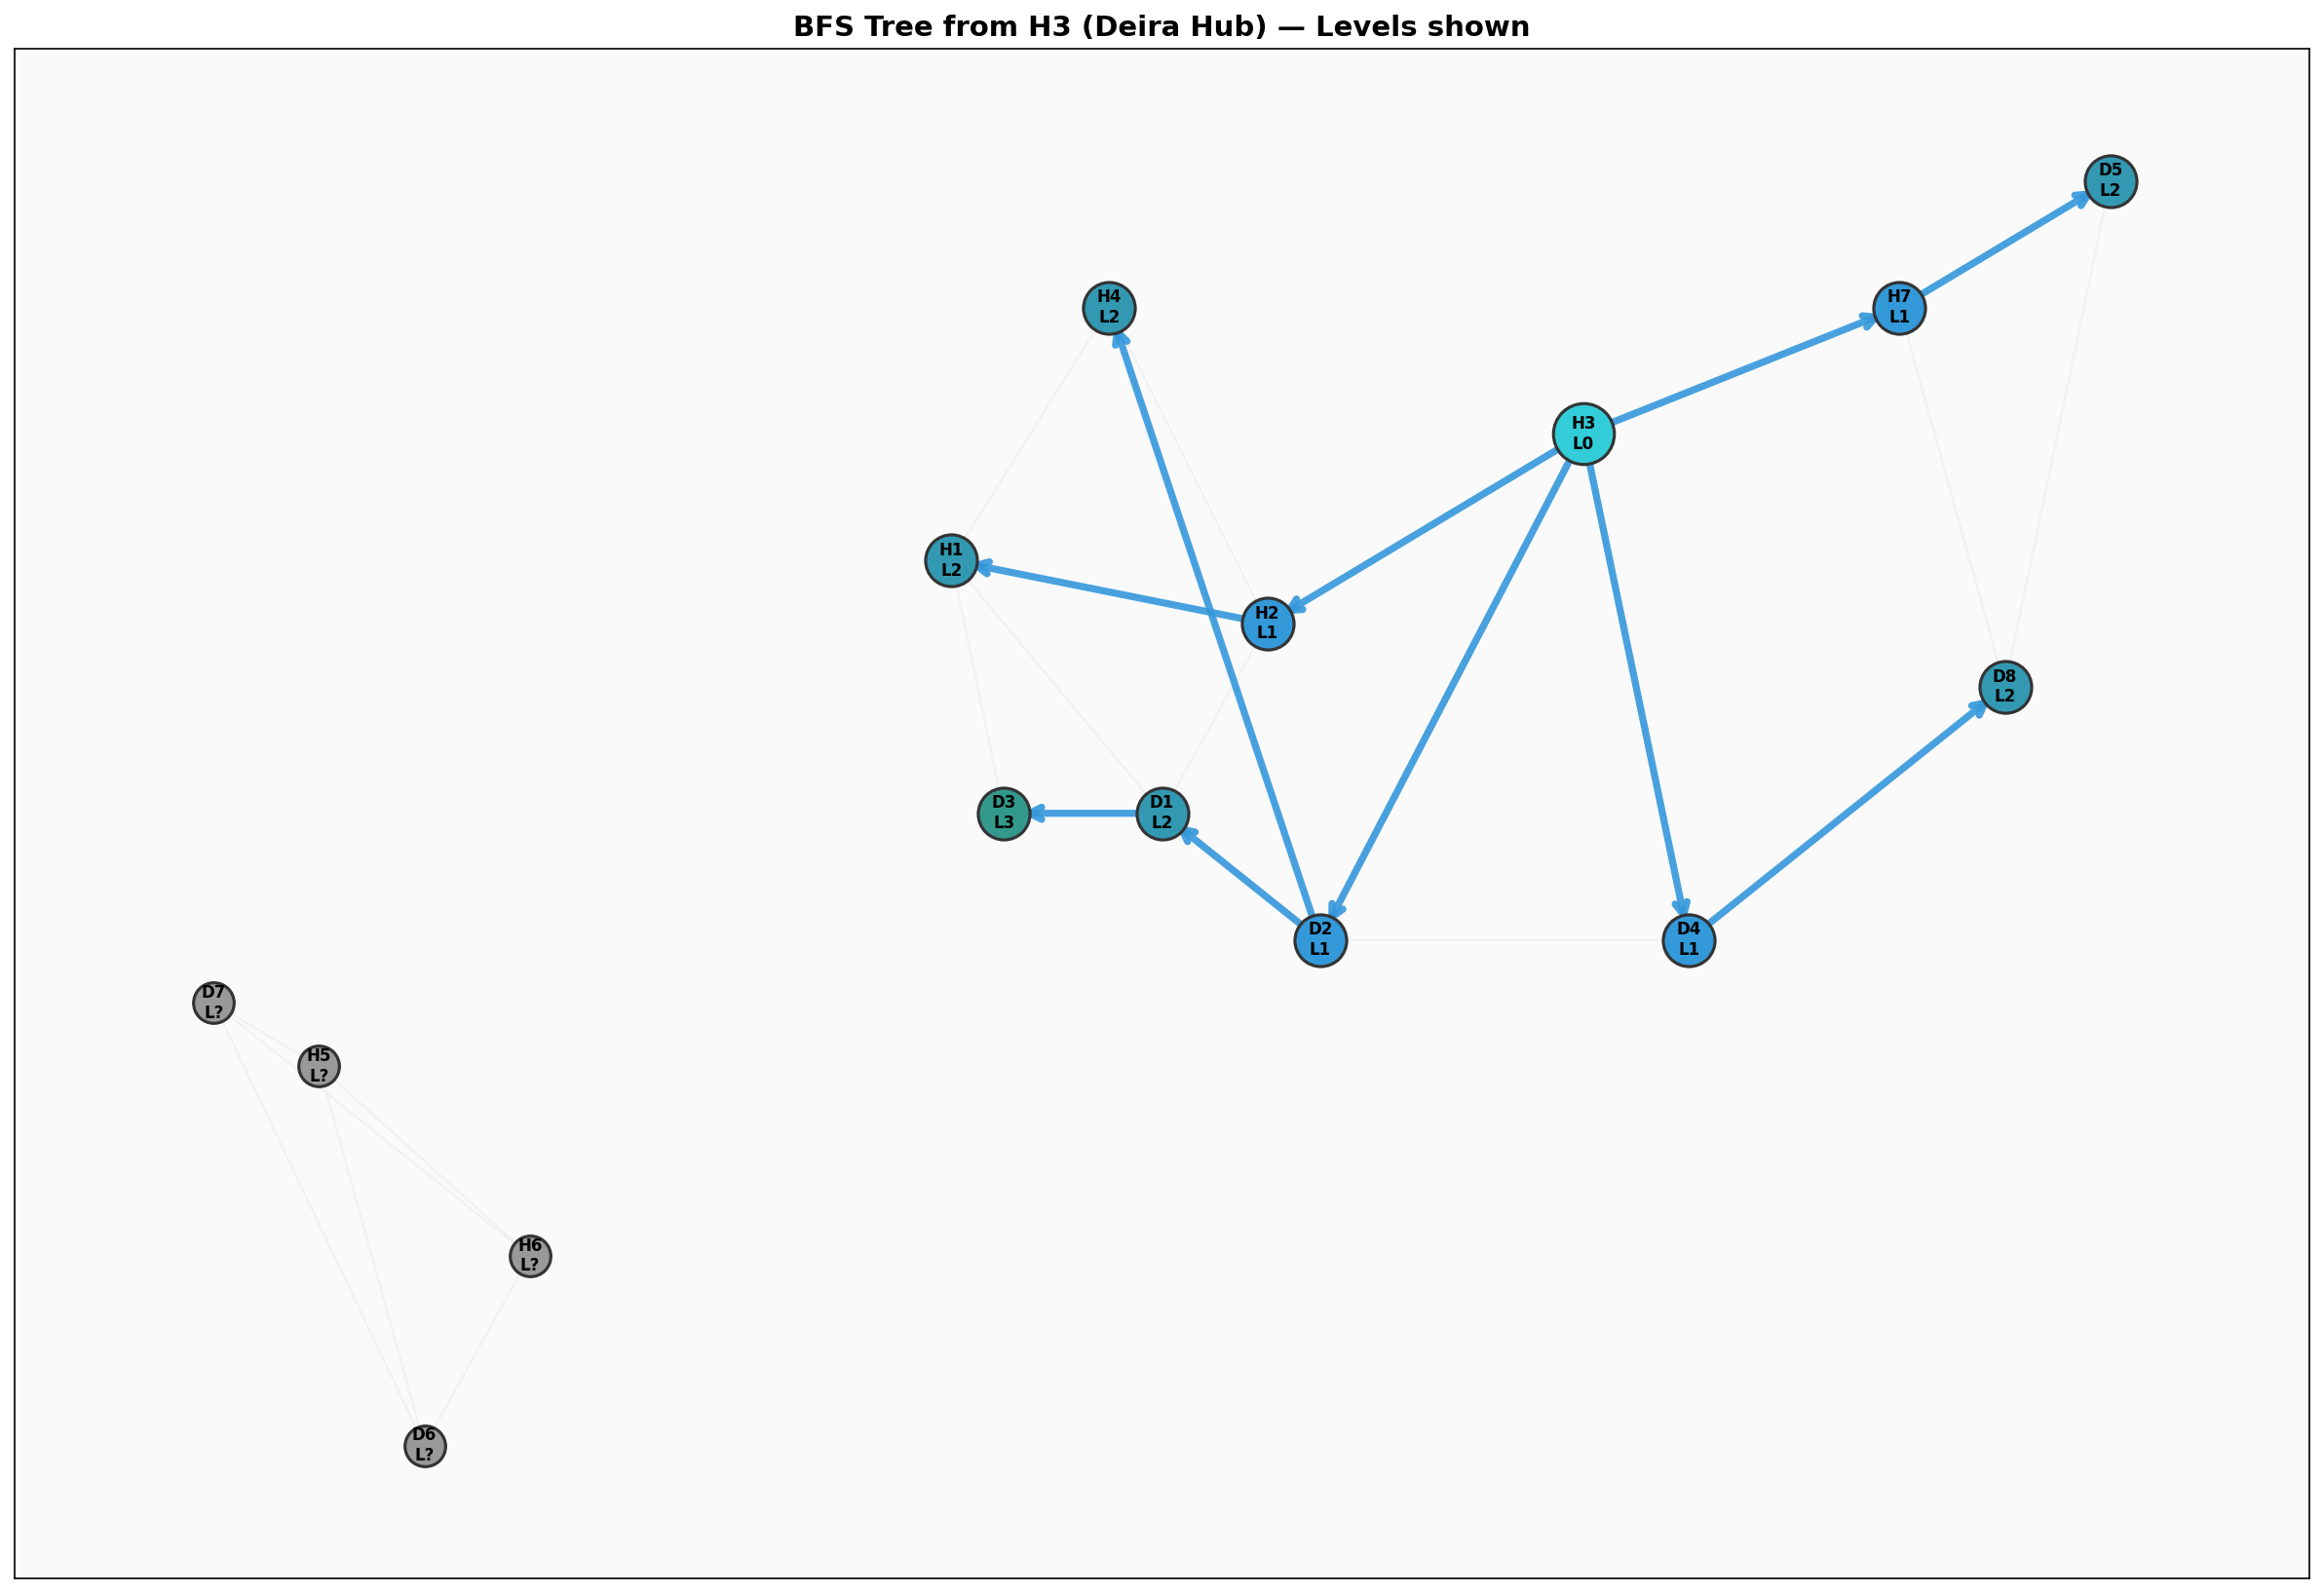
\includegraphics[width=0.85\textwidth]{bfs_tree_h3.png}
\caption{BFS tree from H3 (Deira Hub) with levels indicated}
\label{fig:bfs}
\end{figure}

% ═══════════════════════════════════════════════════════════
% TASK AREA B
% ═══════════════════════════════════════════════════════════
\chapter{Task Area B: Trees, BST \& Balanced Trees}

\section{Q8 --- Binary Search Tree (12 Marks)}

A BST was constructed by inserting 12 Order IDs in the given sequence: 1045, 1023, 1078, 1012, 1034, 1056, 1089, 1005, 1020, 1067, 1050, 1098.

\begin{figure}[H]
\centering
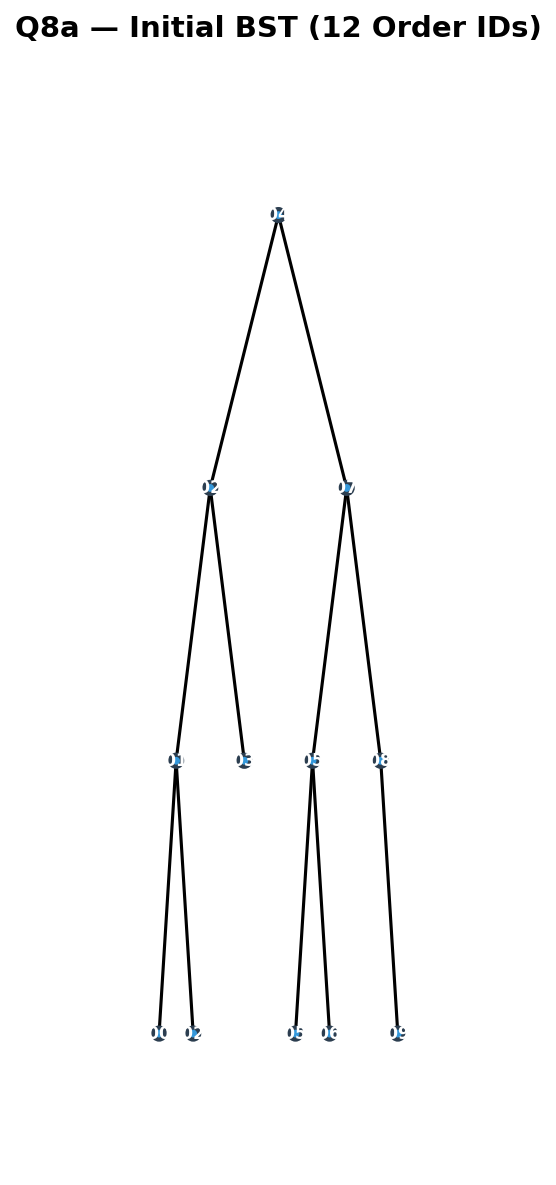
\includegraphics[width=0.48\textwidth]{bst_initial.png}
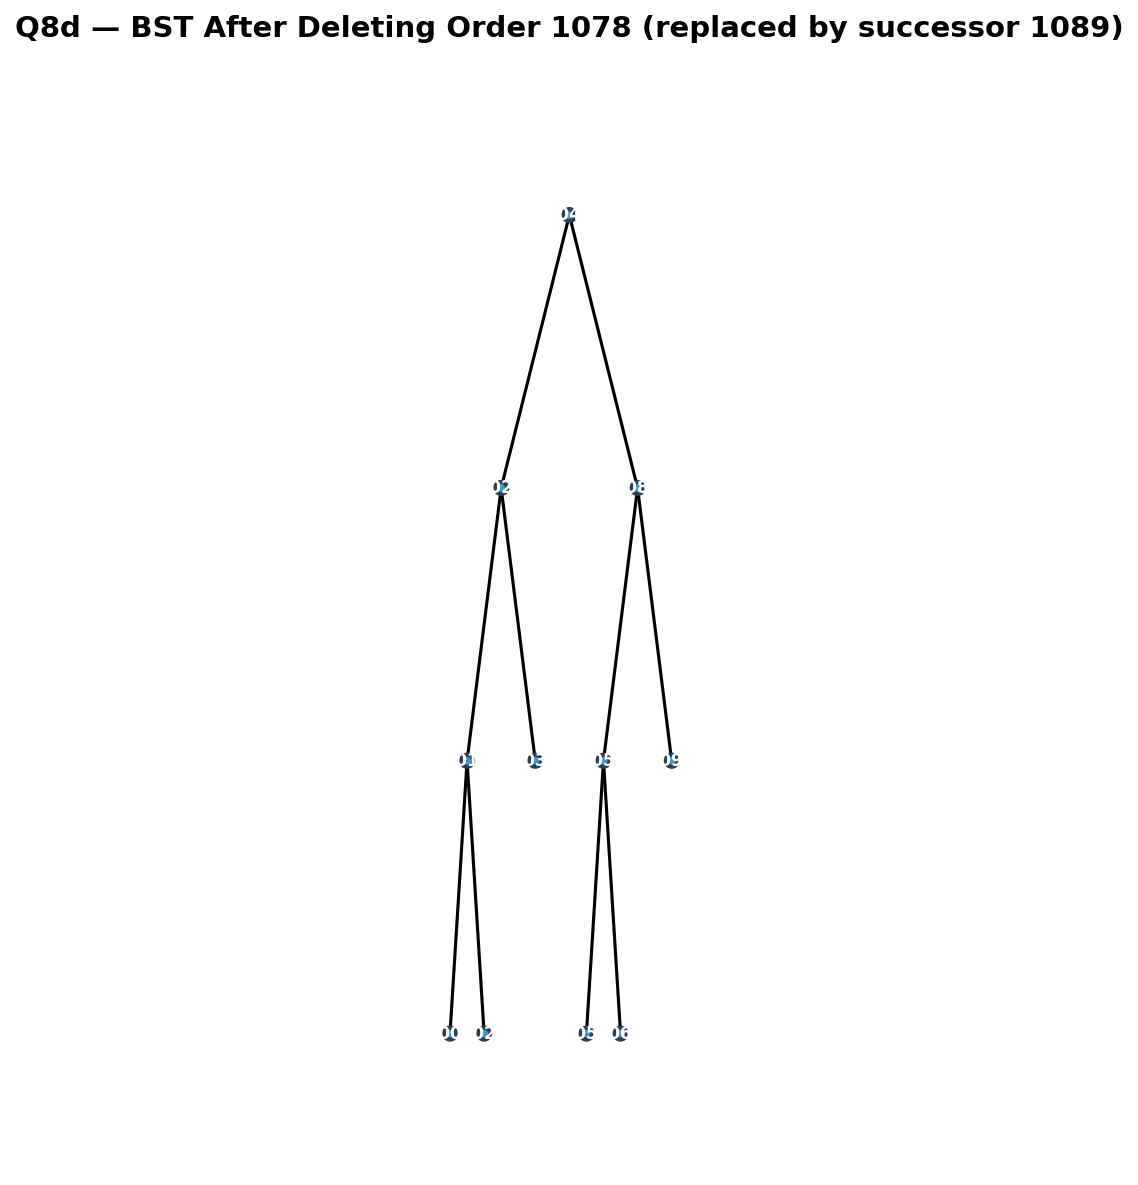
\includegraphics[width=0.48\textwidth]{bst_after_deletion.png}
\caption{BST: initial structure (left) and after deleting Order 1078 (right)}
\label{fig:bst}
\end{figure}

Deletion of Order 1078 (two-children case) was resolved using the in-order successor (1089).

\section{Q9 --- AVL Tree (12 Marks)}

The same 12 Order IDs were inserted into an AVL tree, which performed automatic rotations to maintain balance.

\begin{figure}[H]
\centering
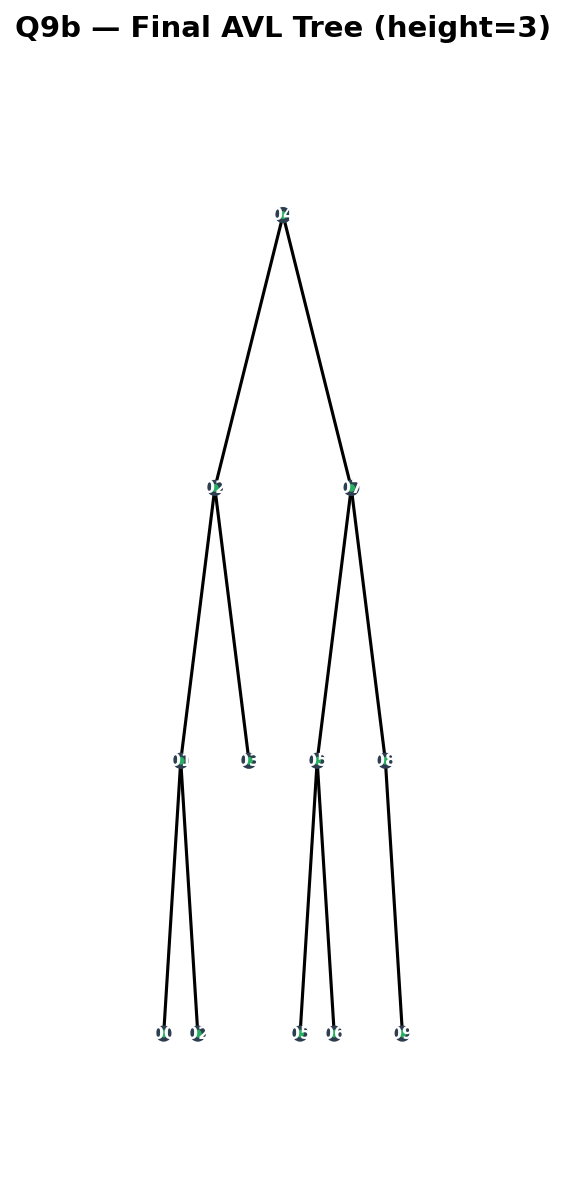
\includegraphics[width=0.7\textwidth]{avl_tree_final.png}
\caption{Final AVL tree after all insertions and rotations}
\label{fig:avl}
\end{figure}

\section{Q10 --- BST vs AVL vs Hash Table (10 Marks)}

AVL tree recommended as the primary order index: guaranteed O($\log n$) insertion and search, plus efficient range queries --- the only structure satisfying all three operational requirements.

\section{Q11 --- Scaling to 15,000 Orders (8 Marks)}

The sorted array bottleneck occurs at $\sim$8,000--10,000 active orders due to O(n) insertion cost. Recommended migration to AVL tree with a three-phase shadow-index rollout plan.

% ═══════════════════════════════════════════════════════════
% TASK AREA C
% ═══════════════════════════════════════════════════════════
\chapter{Task Area C: Linked Lists, Queues \& Order Pipeline}

\section{Q12 --- Doubly Linked List (10 Marks)}
Rider delivery routes modeled as a DLL with O(1) insertion and deletion operations, supporting forward and reverse traversal.

\section{Q13 --- Circular Linked List (8 Marks)}
Round-robin rider assignment using a circular linked list with 8 riders, handling rider removal mid-rotation seamlessly.

\section{Q14 --- Priority Queue with Min-Heap (12 Marks)}
From-scratch min-heap with \texttt{(priority, arrival\_index, order)} tuples ensuring FIFO fairness within equal-priority tiers. VIP orders dispatched first: B$\rightarrow$E$\rightarrow$I (all Priority 1, FIFO preserved).

\section{Q15 --- Stack for Order Lifecycle (8 Marks)}
LIFO stack tracking order status changes with undo capability for accidental dispatch marking.

\section{Q16 --- Dispatch Pipeline Design (10 Marks)}
Per-zone FIFO queues with priority pre-sort recommended over single global queue, with a priority escalation mechanism for cross-zone fairness.

\section{Q17 --- Leadership Brief (10 Marks)}
\memo{TO: CEO \textbar\ FROM: Head of Delivery Operations \textbar\ RE: Priority Queue Implementation}{
Priority dispatch system proposed to address VIP churn (23\% of VIP subscribers lost). Phased rollout: shadow mode (2 weeks) $\rightarrow$ H1 pilot (2 weeks) $\rightarrow$ full network (4 weeks). Projected: 15\% VIP recovery = AED 315,000/year.
}

% ═══════════════════════════════════════════════════════════
% TASK AREA D
% ═══════════════════════════════════════════════════════════
\chapter{Task Area D: Sorting, Searching \& Divide and Conquer}

\section{Q18 --- Merge Sort \& Quick Sort (12 Marks)}
Two-key sort (Zone alphabetical, Priority ascending) implemented from scratch. Merge Sort preferred for stability preserving FIFO order within dispatch groups.

\section{Q19 --- Binary Search vs Linear Search (10 Marks)}
Binary Search finds Order 10347 in $\sim$10 comparisons vs.\ 347 for Linear Search. At 500 daily lookups: 96\% reduction in total comparisons.

\section{Q20 --- Peak Hour Detection (10 Marks)}
Divide-and-conquer approach correctly finds peak ordering hour but is honestly assessed as O(n) --- same as linear scan. Top 3 peak hours identified for staffing optimization.

\section{Q21 --- Sorting Recommendation (8 Marks)}
Merge Sort recommended for 50,000 partially-sorted records: guaranteed O($n \log n$), stable, and naturally suited to pre-sorted runs within zones.

\section{Q22 --- Sorting Performance Simulation (10 Marks)}

\begin{figure}[H]
\centering
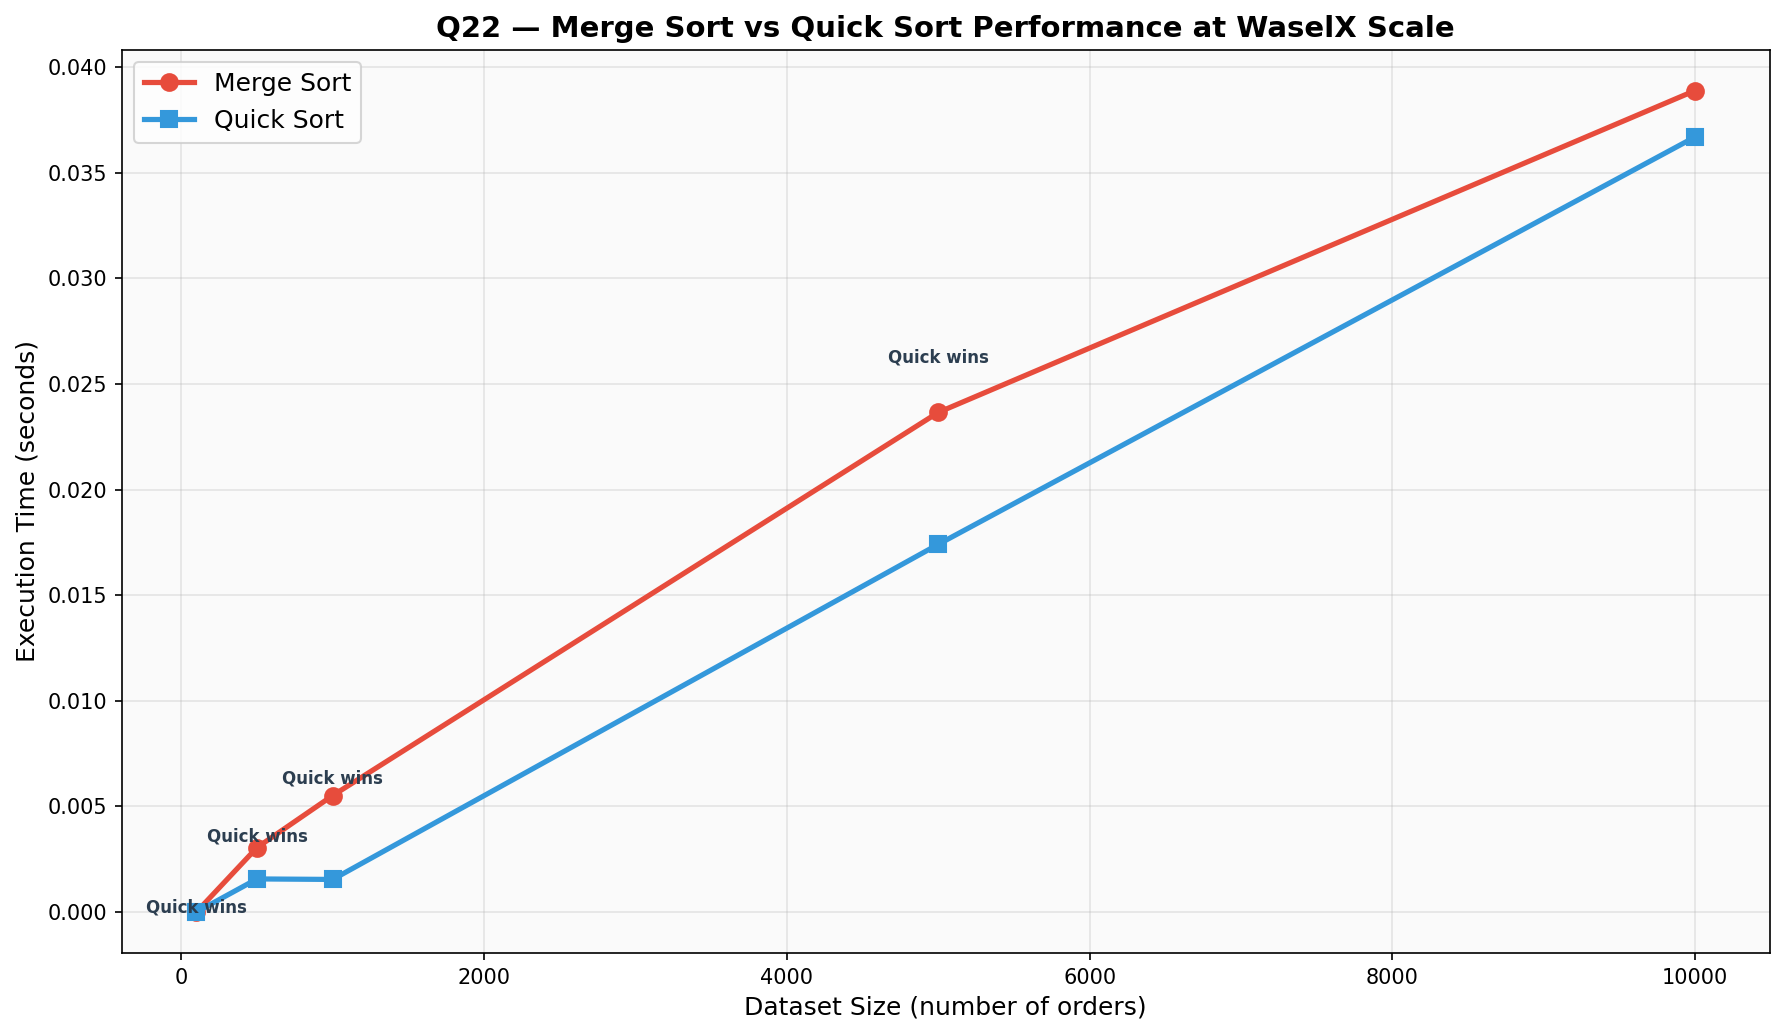
\includegraphics[width=0.8\textwidth]{sorting_performance.png}
\caption{Merge Sort vs Quick Sort execution time across dataset sizes}
\label{fig:sorting}
\end{figure}

% ═══════════════════════════════════════════════════════════
% TASK AREA E
% ═══════════════════════════════════════════════════════════
\chapter{Task Area E: Management, Leadership \& Strategy}

\section{Q23 --- Executive Summary (12 Marks)}
See Chapter 1 for the full 400--500 word executive summary covering all three operational problems, DSA solutions, and prioritized implementation roadmap.

\section{Q24 --- Dual-Audience Communication (10 Marks)}
Route optimization explained for board (analogy-based, business outcomes) and engineering team (complexity analysis, implementation details), with reflection on adaptive communication leadership.

\section{Q25 --- Investment Memo (10 Marks)}
Investment B (priority queue, AED 400K) recommended over Investment A (route optimization, AED 800K) based on identical 50\% ROI, lower capital risk, and strategic alignment with urgent VIP retention needs.

\section{Q26 --- Town Hall Response (10 Marks)}
Response to ``Why not Google Maps?'' addressing cost (AED 790K/year at scale), customization, data ownership, and latency control as strategic justifications for in-house routing capability.

\section{Q27 --- Comprehensive Path Simulator (15 Marks)}

\begin{figure}[H]
\centering
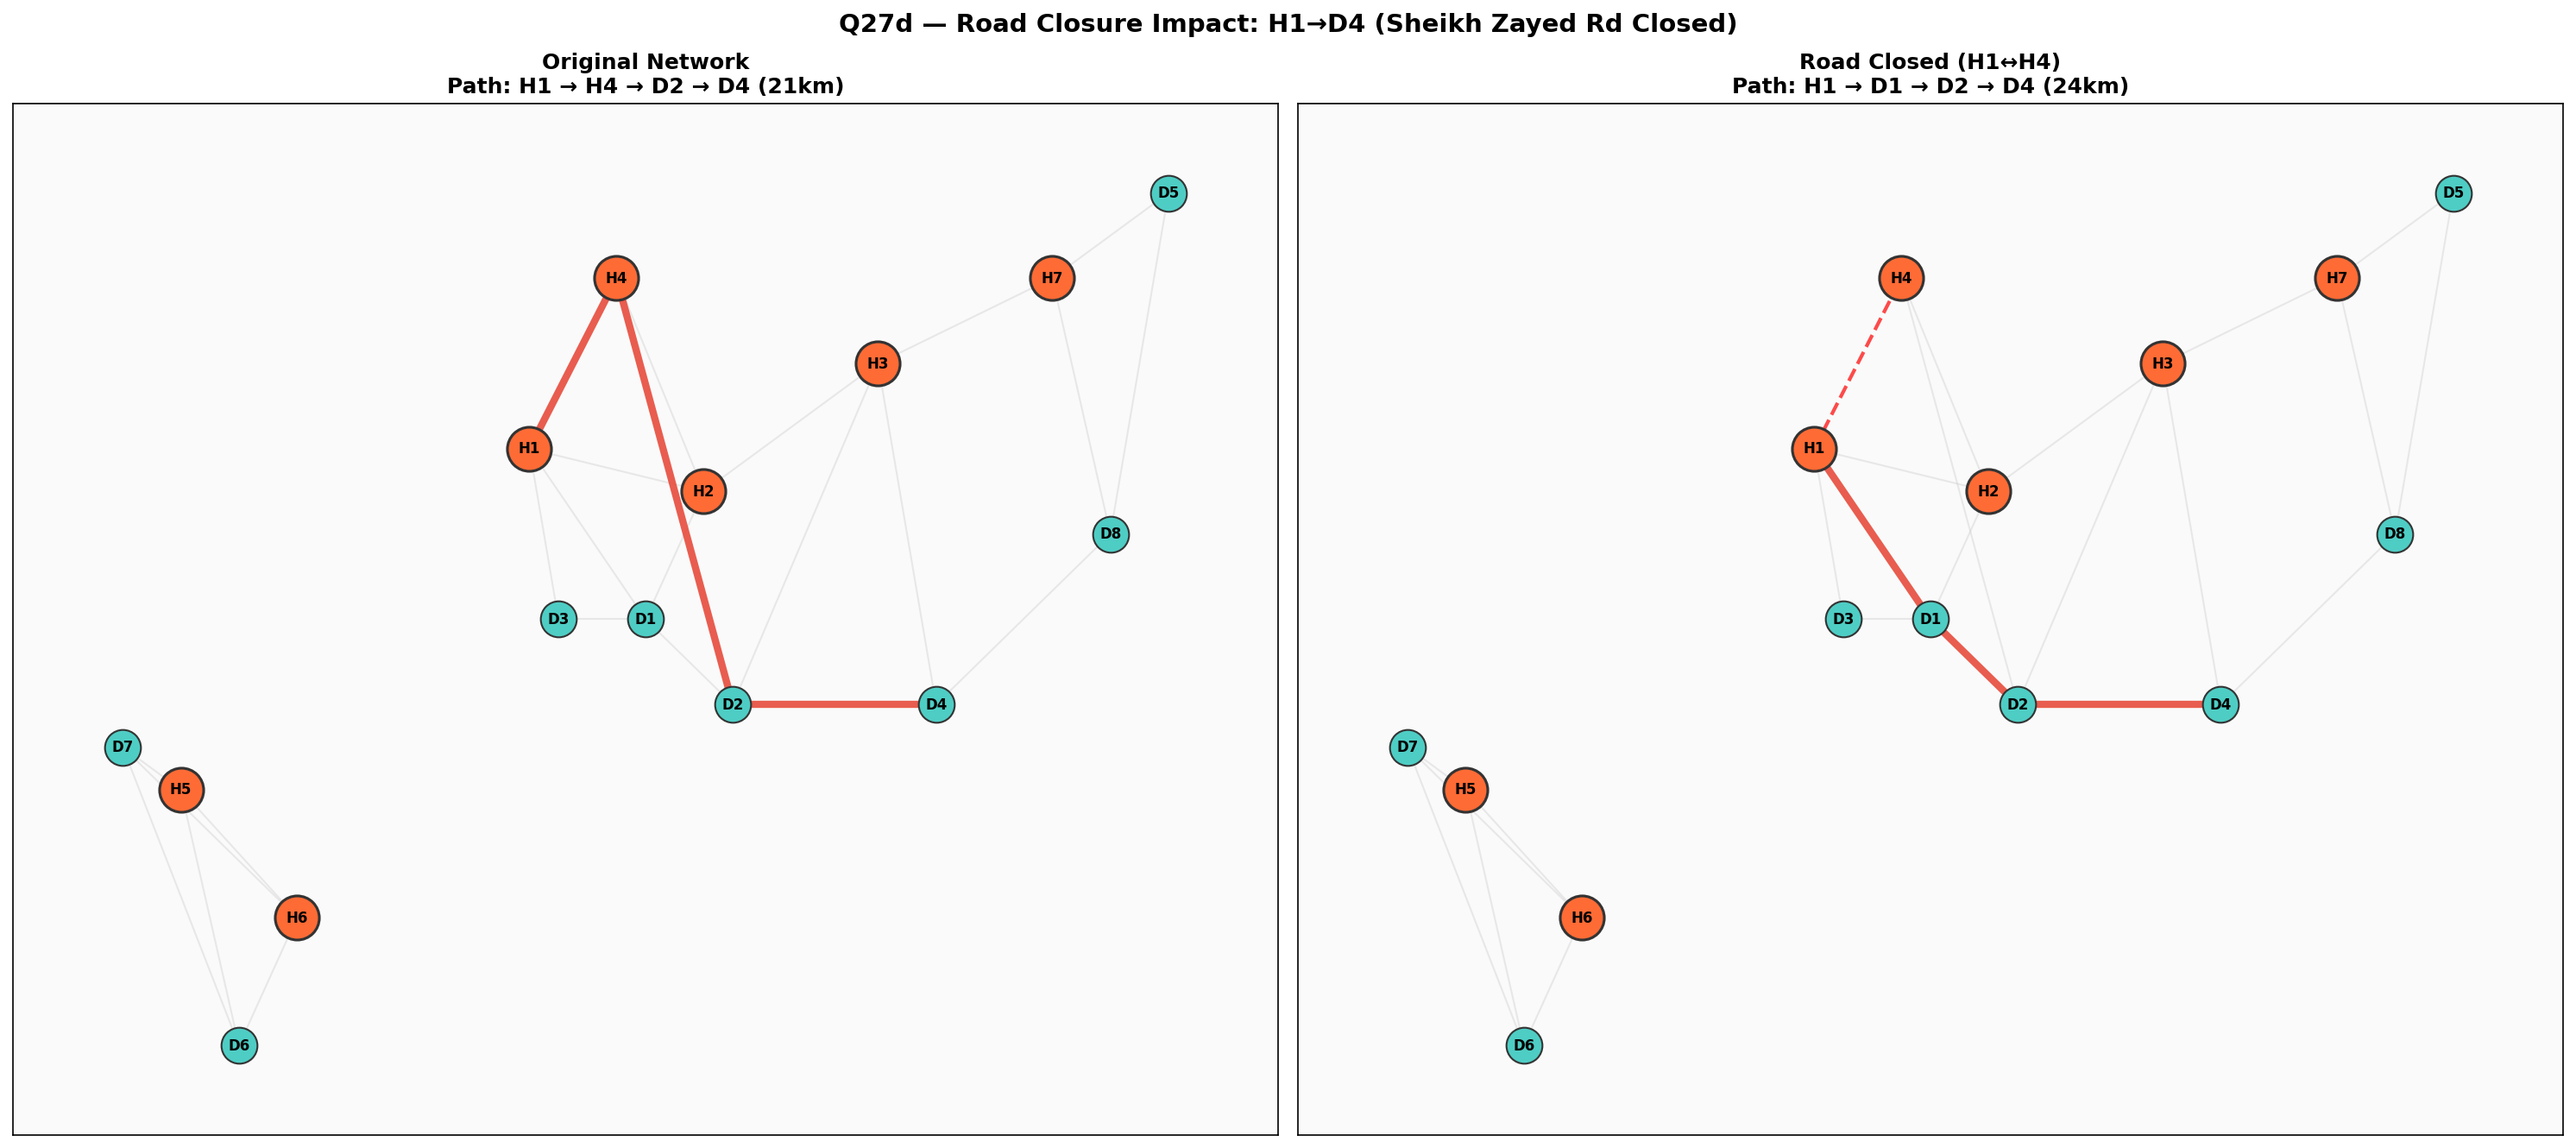
\includegraphics[width=\textwidth]{road_closure_comparison.png}
\caption{Road closure impact: original path vs.\ rerouted path with Sheikh Zayed Rd closed}
\label{fig:closure}
\end{figure}

Full interactive simulator deployed as \texttt{app.py} (Q27 module) with multi-criteria optimization (distance/time/cost) and dynamic road closure simulation.

% ═══════════════════════════════════════════════════════════
% SIMULATION DOCUMENTATION
% ═══════════════════════════════════════════════════════════
\chapter{Simulation Documentation}

A unified Streamlit application (\texttt{app.py}) was developed with two modules:

\begin{itemize}
\item \textbf{Q6 --- Interactive Path Visualizer}: User selects source and destination nodes; Dijkstra computes shortest path by distance; supports overlaying two paths simultaneously.
\item \textbf{Q27 --- Comprehensive Path Simulator}: Multi-criteria optimization (distance, time, cost), road closure toggle, side-by-side comparison with delta analysis.
\end{itemize}

To run locally: \texttt{streamlit run app.py}

GitHub: \url{https://github.com/KartikJoshi23/WaselX-Express}

% ═══════════════════════════════════════════════════════════
% CONCLUSION
% ═══════════════════════════════════════════════════════════
\chapter{Conclusion}

This project demonstrates that well-chosen data structures and algorithms can directly address WaselX Express's three critical operational challenges. Dijkstra's algorithm with a min-heap priority queue provides sub-millisecond route optimization, the AVL tree guarantees consistent O($\log n$) order lookup at scale, and the priority queue dispatch system ensures VIP customers receive service commensurate with their revenue contribution. The projected AED 2.5 million annual benefit against AED 1.2 million implementation cost makes this a compelling technology investment with clear competitive advantages in the UAE last-mile delivery market.

% ═══════════════════════════════════════════════════════════
% REFERENCES
% ═══════════════════════════════════════════════════════════
\chapter*{References}
\addcontentsline{toc}{chapter}{References}

\begin{enumerate}
\item Cormen, T.H., Leiserson, C.E., Rivest, R.L., \& Stein, C. (2022). \textit{Introduction to Algorithms} (4th ed.). MIT Press.
\item Sedgewick, R., \& Wayne, K. (2011). \textit{Algorithms} (4th ed.). Addison-Wesley.
\item Python Software Foundation. (2024). \textit{Python 3.11 Documentation}. \url{https://docs.python.org/3.11/}
\item NetworkX Developers. (2024). \textit{NetworkX Documentation}. \url{https://networkx.org/documentation/}
\item Matplotlib Development Team. (2024). \textit{Matplotlib Documentation}. \url{https://matplotlib.org/stable/}
\item Streamlit Inc. (2024). \textit{Streamlit Documentation}. \url{https://docs.streamlit.io/}
\end{enumerate}

\end{document}
